% !TeX root = ../TFG_LaTeX.tex
\section{Preliminars}

\subsection{El pla complex ampliat. L'esfera de Riemann}

\begin{adjustwidth}{1cm}{1cm}

Coneguts ja els nombres complexos i el pla complex $\mathbb{C}$, es té que la correspondència 
$$z=x+iy \longleftrightarrow (x,y)$$
és una bijecció entre $\mathbb{C}$ i el pla Euclidià $\mathbb{R}^2$.

La topologia de $\mathbb{C}$ coincideix amb la de $\mathbb{R}^2$, és a dir, dotem $\mathbb{C}$ amb la topologia usual que ve de la mètrica euclidiana.
    
\begin{definicio}

    Es defineix el \textbf{pla complex ampliat} com el conjunt
    \[
        \mathbb{C}^* = \mathbb{C} \cup \{\infty\},
    \]
    on $\infty$ és un punt addicional anomenat \textbf{punt a l'infinit} que de manera intuitiva pot ser vist com el límit de qualsevol punt no nul quan fem tendir el seu mòdul a infinit.
    \label{pla_complex_ampliat}
\end{definicio}

L'aritmètica de $\mathbb{C}^*$ té algunes particularitats respecte de la de $\mathbb{C}$. Si $z,w\neq \infty$, aleshores totes les propietats de $\mathbb{C}$ funcionen exactament en $\mathbb{C}^*$ per a $z,w$. Ara bé, tenim que
\[
\begin{array}{rcll}
z+\infty &=& \infty+z=\infty,
& z\in\mathbb C, \\[4pt]

z\cdot\infty &=& \infty\cdot z=\infty,
& z\in\mathbb C\setminus\{0\}, \\[4pt]

\dfrac{z}{\infty} &=& 0,
& z\in\mathbb C, \\[8pt]

\dfrac{z}{0} &=& \infty,
& z\in\mathbb C\setminus\{0\}, \\[8pt]

\dfrac{\infty}{z} &=& \infty,
& z\in\mathbb C\setminus\{0\}.
\end{array}
\]

La topologia estàndard de $\mathbb{C}^*$ és la que està formada pels conjunts oberts de $\mathbb{C}$ amb la topologia habitual euclidiana (veient $\mathbb{C}$ com $\mathbb{R}^2$) i també pels conjunts de la forma $\{\mathbb{C}^*\backslash K:K\subset \mathbb{C}\text{ és compacte}\}$. Els primers seran entorns dels punts en $\mathbb{C}$, i els segons seran entorns del punt a l'infinit. Denotarem aquesta topologia per $\mathcal{G}_{\infty}$.

Recordem que es denota $S^2$ a la esfera unitat $\{(x,y,z)\in \mathbb{R}^3 : x^2+y^2+z^2=1\}$, és a dir, l'esfera de radi 1 centrada en el punt $(0,0,0)$.

Com $S^2$ es considera un subespai de $\mathbb{R}^3$, la seua topologia és la topologia induïda de la usual de $\mathbb{R}^3$, l'euclidiana.

Una manera de visualitzar $\mathbb{C}^*$ és mitjançant la projecció estereogràfica. Aquesta és una funció que transforma l'esfera unitat $S^2$ de l'espai euclidià tridimensional $\mathbb{R}^3$ en el pla complex ampliat, que es defineix de la manera següent.

Siga $P = (X,Y,Z)$ qualsevol punt de l'esfera unitat diferent del pol nord $N = (0,0,1)$. Es traça la recta que passa per $N$ i $P$, i definim la \textbf{projecció estereogràfica} de $P$ com el punt $z=x+iy$ de $\mathbb{C}^*$ de manera que la recta anterior talla al pla de coordenades $Z=0$ al punt $(x,y,0)$.

La projecció estereogràfica del pol nord $N$ ve donada pel punt de l'infinit $\infty$ de $\mathbb{C}^*$.

\begin{figure}[H]
    \centering
    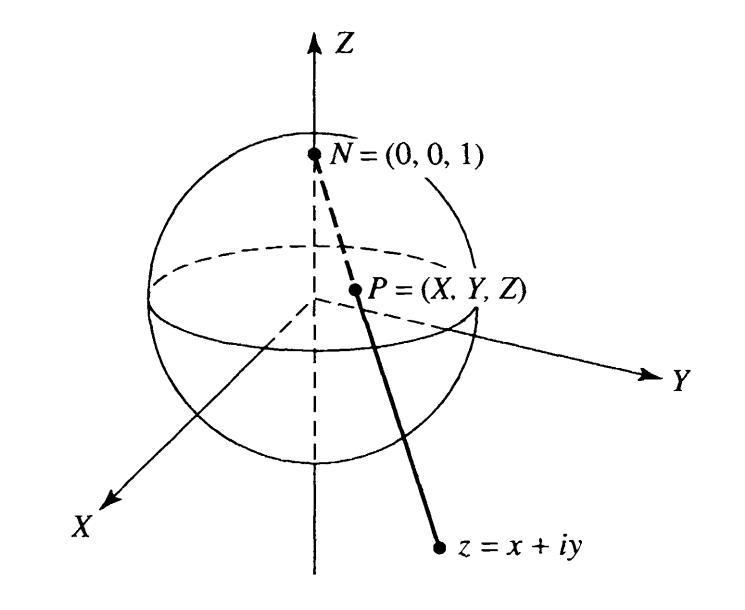
\includegraphics[width=0.35\textwidth]{pictures/Projeccio_Estereografica.png}
    \begin{adjustwidth}{1cm}{1cm}
       \caption{Projecció estereogràfica.}
    \label{fig:proj_est} 
    \end{adjustwidth}
\end{figure}

Analíticament, la projecció estereogràfica pren l'expressió 
\[
    \pi: S^2 \to \mathbb{C}^*, \quad \pi(X,Y,Z)=
    \begin{cases}
        \frac{X+iY}{1-Z}, &\text{ si }(X,Y,Z)\neq (0,0,1)\\
        \;\;\infty, &\text{ si }(X,Y,Z)=(0,0,1)
    \end{cases}
\] 
i, anàlogament, la seua inversa ve donada per l'expressió 
\[
    \pi^{-1}(z)=\left(\frac{2\operatorname{Re}(z)}{|z|^2+1},\frac{2\operatorname{Im}(z)}{|z|^2+1},\frac{|z|^2-1}{|z|^2+1} \right).
\]

%El punt $(X,Y,Z)$ de l'esfera queda determinat de manera única pel punt $z = x + iy$ del pla. Així, la projecció estereogràfica proporciona una bijecció entre els punts $P$ de l'esfera i els punts $z = x + iy$ del pla complex, exceptuant només el pol nord $N=(1,0,0)$, que es correspon amb el punt a l'infinit com ja s'ha mencionat.

Els meridians sobre l'esfera corresponen a rectes del pla que passen per $0$, mentre que les línies de latitud corresponen a circumferències centrades en $0$. A mesura que els radis d'aquestes circumferències tendeixen a $\infty$, les línies de latitud de l'esfera s'aproximen al pol nord. Per tant, és natural fer correspondre el pol nord $N$ amb el punt a l'infinit.  

És degut a aquesta bijecció entre l'esfera $S^2$ i el pla complex ampliat, que aquest últim també rep el nom d'\textbf{esfera de Riemann}.

És ben conegut que $\mathbb{C}^*$ i $S^2$ són homeomorfs amb les topologies que hem descrit anteriorment, i ho denotarem com $\mathbb{C}^*\cong S^2$.

%Per tant, comprobem que la topologia $\mathcal{G}_{\infty}$ que havíem donat per a $\mathbb{C}^*$ és coherent amb aquesta identificació, ja que una base d'entorns de $N$ en la topologia de $S^2$ està formada pels conjunts de la forma $\{B(N, \varepsilon): \varepsilon>0\}\cap S^2$, i quan transformem per la projecció estereogràfica $S^2$ en $\mathbb{C}^*$, la base queda transformada en la base de entorns del punt a l'infinit (que és el que correspón a $N$) $\{\mathbb{C}^*\backslash \overline{B}(0,\varepsilon) : \varepsilon>0\}$, i resulta que això genera exactament els oberts (els que són entorns de $\infty$) que havíem dit que formaven la topologia de $\mathbb{C}^*$.

\begin{subsection}{Diferenciabilitat en \texorpdfstring{$\mathbb{R}^2$}{C} }

Anem a recordar algunes nocions bàsiques de diferenciabilitat en $\mathbb{R}^2$.

\begin{definicio}
Siga $U\subset \mathbb{R}^2$ un obert i siga
\[
f:U\longrightarrow \mathbb{R}^2
\]
una aplicació. Direm que $f$ és \textbf{diferenciable} en un punt
$p=(x_0,y_0)\in U$ si existeix una aplicació lineal
\[
Df(p):\mathbb{R}^2\longrightarrow \mathbb{R}^2
\]
tal que
\[
\lim_{h\to 0}
\frac{\|f(p+h)-f(p)-Df(p)(h)\|}{\|h\|}=0.
\]
L'aplicació lineal $Df(p)$ s'anomena \textbf{diferencial} de $f$ en $p$.
Direm que $f$ és diferenciable en $U$ si ho és en tots els punts de $U$.
\end{definicio}

\begin{definicio}
Si escrivim
\[
f(x,y)=(u(x,y),v(x,y)),
\]
les funcions $u$ i $v$ s'anomenen les \textbf{components} de $f$. Les \textbf{derivades
parcials de $f$} són les derivades parcials de les seues components:
\[
\frac{\partial u}{\partial x},\qquad
\frac{\partial u}{\partial y},\qquad
\frac{\partial v}{\partial x},\qquad
\frac{\partial v}{\partial y}.
\]
A més, gastarem la notació 
\[
D_1u:=\frac{\partial u}{\partial x},\qquad
D_1v:=\frac{\partial v}{\partial x},\qquad
D_2u:=\frac{\partial u}{\partial y},\qquad
D_2v:=\frac{\partial v}{\partial y}.
\]
\end{definicio}

\begin{definicio}
Siga $U\subset \mathbb{R}^2$ un obert. Direm que una aplicació
$f:U\to\mathbb{R}^2$, $f=(u,v)$, és de \textbf{classe $\mathcal{C}^1$} en $U$ si
les derivades parcials $
D_1u,D_1v,D_2u,D_2v$
existeixen en tots els punts de $U$ i són contínues en $U$.
\end{definicio}

\begin{nota}
Si $f:U\to\mathbb{R}^2$ és de classe $\mathcal{C}^1$, aleshores $f$ és
diferenciable en $U$. En aquest cas, per a cada punt $(x_0,y_0)\in U$, la matriu
associada a la diferencial $Df(x_0,y_0)$ en les bases canòniques és
\[
\begin{pmatrix}
D_1u(x_0,y_0) &
D_2u(x_0,y_0) \\[1.2ex]
D_1v(x_0,y_0) &
D_2v(x_0,y_0)
\end{pmatrix}.
\]
Aquesta matriu s'anomena \textbf{matriu jacobiana} de $f$ en el punt
$(x_0,y_0)$.
\end{nota}

\begin{nota}
Denotarem per $J_f(x_0,y_0)$ el \textbf{jacobià} de $f$ en el punt
$(x_0,y_0)$, és a dir, el determinant de la matriu jacobiana:
\[
J_f(x_0,y_0)=
\det
\begin{pmatrix}
D_1u(x_0,y_0) &
D_2u(x_0,y_0) \\[1.2ex]
D_1v(x_0,y_0) &
D_2v(x_0,y_0)
\end{pmatrix}.
\]

\end{nota}

\end{subsection}

\subsection{Funcions holomorfes}
    
\begin{nota}
    Normalment $U\subset \mathbb{C}$ denotarà un conjunt obert de $\mathbb{C}$ durant el treball.
\end{nota}

\begin{definicio}
    Siga $U\subset \mathbb{C}$, i siga $z_0\in U$. Direm que la funció complexa $f:U\to \mathbb{C}$ és \textbf{derivable} en $z_0$ si existeix
    \begin{equation}
        \lim_{z\to z_0} \frac{f(z)-f(z_0)}{z-z_0},
        \label{eqquodif}
    \end{equation}
    i aquest límit es denota per $f'(z_
    0)$ o per $\frac{df}{dz}(z_0)$, que anomenem \textbf{derivada} de $f(z)$ en $z_0$.

    A més, una funció $f(z)$ es diu que és \textbf{holomorfa en l'obert} $U \subset \mathbb{C}$ si $f(z)$ és derivable en cada punt de $U$. És ben conegut que una funció és holomorfa si i només si és analítica, és a dir, si es pot desenvolupar localment en sèrie de potències i, per tant, els dos conceptes són equivalents en el context complex.
\end{definicio}

\begin{exemple}
    La funció $f(z)=2z+1$, definida en tot $\mathbb{C}$, és derivable per a qualsevol $z\in \mathbb{C}$, ja que si $z_0\in \mathbb{C}$, 
    \[
        \lim_{z\to z_0} \frac{f(z)-f(z_0)}{z-z_0}= \lim_{z\to z_0} \frac{2z+1-(2z_0+1)}{z-z_0}=\lim_{z\to z_0}2\frac{z-z_0}{z-z_0}=2,
    \]
    i per a tot $z\in \mathbb{C}$ la seua derivada complexa és $f'(z)=2$.
\end{exemple}

\begin{nota}
    És ben conegut que si $f(z)$ és derivable en $z_0$, aleshores $f(z)$ és contínua en $z_0$.
\end{nota}


\begin{teorema}[Equacions de Cauchy-Riemann]
    Siga $U \subset \mathbb{C}$, i $f:U \to \mathbb{C}$ una funció definida per
    \[
        f(x+iy)=u(x,y)+iv(x,y),
    \]
    on $u,v:U \to \mathbb{R}$ són les seues parts real i imaginària, respectivament. Si $z_0=x_0+iy_0\in U$, aleshores són equivalents:

    \begin{enumerate}
        \item $f$ és derivable complexa en el punt $z_0$
        \item La corresponent $f:U\subset \mathbb{R}^2\to \mathbb{R}^2$ definida per $f(x,y)=(u(x,y),v(x,y))$ és diferenciable real en $(x_0,y_0)$ i es compleixen les equacions de Cauchy-Riemann: 
    \end{enumerate}
    \[
        \frac{\partial u}{\partial x}(x_0,y_0)
        =
        \frac{\partial v}{\partial y}(x_0,y_0),
        \qquad
        \frac{\partial u}{\partial y}(x_0,y_0)
        =
        -\frac{\partial v}{\partial x}(x_0,y_0).
    \]

    En el cas que $f$ siga derivable en $z_0$ es compleix
    \[
        f'(z_0)=\frac{\partial u}{\partial x}(x_0,y_0)+i\frac{\partial v}{\partial x}(x_0,y_0)=\frac{\partial f}{\partial x}(x_0,y_0)
    \]
    \label{cauchy_riemann}
\end{teorema}

A continuació recordem la regla de la cadena per a funcions complexes, que emprarem més avant.

\begin{teorema}[Regla de la cadena]
    Siguen $U,V$ oberts de $\mathbb{C}$, $f:V\subset \mathbb{C}\to \mathbb{C}$ i $g:U\subseteq \mathbb{C}\to \mathbb{C}$ de forma que $g(U)\subseteq V$, i siguen $z_0\in U, w_0=g(z_0)\in V$.

    Si $g$ és diferenciable en $z_0\in U$, i $f$ és diferenciable en $w_0=g(z_0)\in V$, aleshores la composició $(f \circ g)(z) = f(g(z))$ és diferenciable en $z_0$ i 
    \begin{equation}
        (f \circ g)'(z_0) = f'(g(z_0))g'(z_0).
    \end{equation}
    \label{reglacadena}
\end{teorema}

\begin{exemple}
    Siguen $g(z)=3z+2$ i $f(z)=z^2$, ambdues funcions definides en tot $\mathbb{C}$. Les dues són diferenciables en tot $\mathbb{C}$, i si $z_0\in \mathbb{C}$, aleshores 
    \[
        (f\circ g)'(z_0)=f'(g(z_0))g'(z_0)=3(2(3z_0+2))=18z_0+12
    \]
\end{exemple}

Anem a recordar ara resultats clàssics d'anàlisi.

\begin{teorema}[Principi dels zeros aïllats]
    Siga $U\subset \mathbb{C}$ un obert i connex de $\mathbb{C}$. Siga $f:U\to \mathbb{C}$ una funció holomorfa que no és idènticament nul·la. Si $f(z_0)=0$ per a $z_0\in U$ aleshores existeix un $\varepsilon>0$ tal que $f(z)\neq 0$ per a tot $0<|z-z_0|<\varepsilon$.
    \label{zeros_aillats}
\end{teorema}

\begin{teorema}[de l'aplicació oberta]
    Siga $U\subset \mathbb{C}$ un obert i connex de $\mathbb{C}$, i siga $f:U\to \mathbb{C}$ una funció holomorfa no constant. Aleshores, per a qualsevol obert $A\subset U$, es té que $f(A)$ és obert.
    \label{teo_apl_oberta}
\end{teorema}

\begin{teorema}[Teorema del Mòdul Màxim]
        Si $f$ és una funció holomorfa en l'obert connex $G$ i $a\in G$ tal que $|f(a)|\geq |f(z)|$ per a tot $z$ en $G$, aleshores $f$ ha de ser constant.
        \label{teo_mod_max}
    \end{teorema}

    %\begin{proof}
        %Comencem denotant $\Omega=f(G)$, i siga $\alpha=f(a)$. Per hipòtesi tenim que $|\alpha|\geq |\xi|$ per a tot $\xi$ en $\Omega$. Ara, per el principi anterior, tenim que $\alpha$ es troba en $\partial\Omega\cap\Omega$, cosa que impideix que $\Omega$ siga obert. Conseqüentment, pel teorema de l'aplicació oberta, $f$ ha de ser constant.
    %\end{proof}

També podem enunciar una conseqüencia d'aquest teorema.

\begin{teorema}
    Si $G$ és un conjunt obert i fitat en $\mathbb{C}$ i $f$ és una funció contínua en $\overline{G}$ que és holomorfa en $G$, aleshores 
    \[
        \max\{|f(z)|:z\in\overline{G}\}=\max\{|f(z)|:z\in\partial G\},
    \]
    on $\partial G$ denota la frontera de $G$.
    \label{conseq_teo_mod_max}
\end{teorema}

És a dir, baix les condicions exigides, el valor absolut de la funció sempre pren el seu màxim en la frontera de l'obert.

\begin{teorema}[de Vitali]
    Siga $U\subseteq \mathbb{C}$ un obert, i siga $\{f_n\}$ una successió de funcions holomorfes en $U$. Si la successió $\{f_n\}$ està localment acotada en $U$, és a dir, que per a tot $K\subset U$ compacte existeix una constant $M_k>0$ de forma que $|f_n(z)|\leq M_k$ per a tot $z\in K$ i per a tot $n\in\mathbb{N}$, i a més la successió $\{f_n\}$ convergeix puntualment en $U$ a una funció $f$, aleshores la successió $\{f_n\}$ convergeix a $f$ uniformement sobre qualsevol subconjunt compacte de $U$, i per tant, $f$ és holomorfa en $U$.

    Podem trobar aquest teorema, la seua prova i més informació relacionada en \cite[Cap. VII, Secció 2]{conway}.
    \label{vitali}
\end{teorema}

Recordem també el teorema que pot ser trobat en \cite[p. 99]{conway}:

\begin{teorema}
    Siguen $U,V$ oberts connexos de $\mathbb{C}$, i siga $f$ una bijecció holomorfa entre $U$ i $V$. Aleshores es té que $f^{-1}$ també és holomorfa.
    \label{bij_holo_te_inv_holo}
\end{teorema}

%\begin{proof}
    %Com $G$ és fitat, existeix un punt punt $a\in\overline{G}$ tal que $|f(a)|\geq |f(z)|$ per a tot $z\in\overline{G}$. Si $f$ és una funció constant la conclusió és trivial, així que suposem que $f$ no és constant. Tenim que $a$ ha d'estar en una component connexa de $\overline{G}$. Aleshores pel teorema (\ref{teo_mod_max}) $a$ no pot estar en l'interior d'eixa component connexa perquè si no, $f$ hauria de ser constant. Per tant, $a$ ha d'estar en la seua frontera, i per tant en $\partial G$.
%\end{proof}

\begin{definicio}
    Denotarem com $\mathbb{D}$ al disc unitat obert, que ve donat pel conjunt $\{z\in \mathbb{C}: |z|<1\}$. De forma coherent, denotarem $\overline{\mathbb{D}}=\{z\in \mathbb{C}: |z|\leq 1\}$ al disc unitat tancat, $\mathbb{D}^*=\mathbb{D}\backslash \{0\}$ al disc unitat foradat, i $\partial\mathbb{D}=\overline{\mathbb{D}}\backslash\mathbb{D}$  a la frontera del disc unitat.
\end{definicio}

%\begin{proof}
    %Recordem que en general, la derivada direccional de $f: U \to \mathbb{C}$ en el punt $a\in U$ i en la direcció $v\in\mathbb{C}$ es defineix com 
    %\[
        %D_vf(a):=\lim_{t \to 0}\frac{f(a+tv)-f(a)}{t},
    %\]    
        %i que si $f$ és diferenciable, aleshores admet derivada direccional en totes direccions, i 
   %\[
        %D_vf(a)=Df(a)(v)=\nabla f(a)\cdot \begin{pmatrix}
           % v_1 \\
           % v_2
        %\end{pmatrix}, 
    %\] 
    %on $Df(a)$ és el diferencial de $f$ en $a$, i $\nabla f$ és el gradient de $f$.

   % Així doncs, com $\nabla h = 0$, la derivada direccional de $h(x,y)$ en qualsevol direcció és 0. Per tant, $h(x,y)$ és constant en qualsevol segment contingut en $D$, i per tant, en qualsevol polígonal en $D$. 
    
    %Ara bé, com $D$ és connex, qualssevol 2 punts de $D$ es poden unir mitjançant una poligonal dins del conjunt. Això prova que $h$ és constant en $D$.
%\end{proof}

Recordem algunes definicions de conjunts:

\begin{definicio}
    Un conjunt és \textbf{convex} si per a tot parell de punts en el conjunt, el segment que els uneix queda dins del conjunt.

    Formalment, un conjunt $A\subset \mathbb{C}$ es diu que és convex si per a tot $z_1,z_2\in A$ es compleix que $tz_1+(1-t)z_2$ està en $A$ per a $t\in (0,1)$.

    A més, un conjunt és \textbf{estrel·lat respecte a} $z_0$ si per a qualsevol punt del conjunt, el segment que l'uneix amb $z_0$ queda dins del conjunt.

    De manera formal, es diu que $A\subset \mathbb{C}$ és estrel·lat respecte a $z_0\in A$ si per a tot $z\in A$, es compleix que $tz_0+(1-t)z$ està en $A$ per a $t\in (0,1)$.
\end{definicio}

\begin{figure}[H]
    \centering

    \begin{subfigure}{0.50\textwidth}
        \centering
        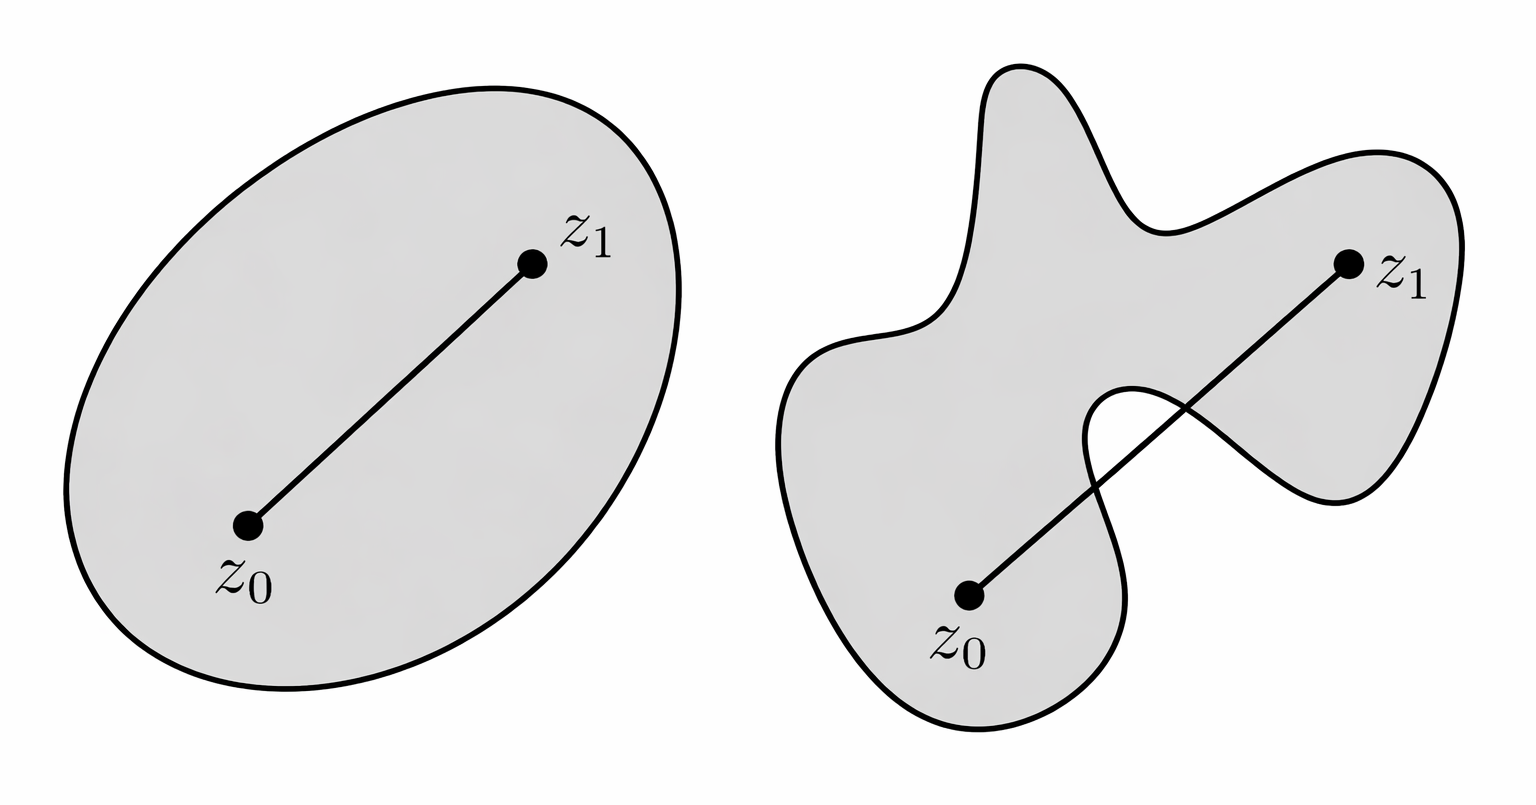
\includegraphics[width=\linewidth]{pictures/convex.png}
        \caption{Conjunt convex i conjunt no convex}
        \label{fig:convex}
    \end{subfigure}
    \hfill
    \begin{subfigure}{0.25\textwidth}
        \centering
        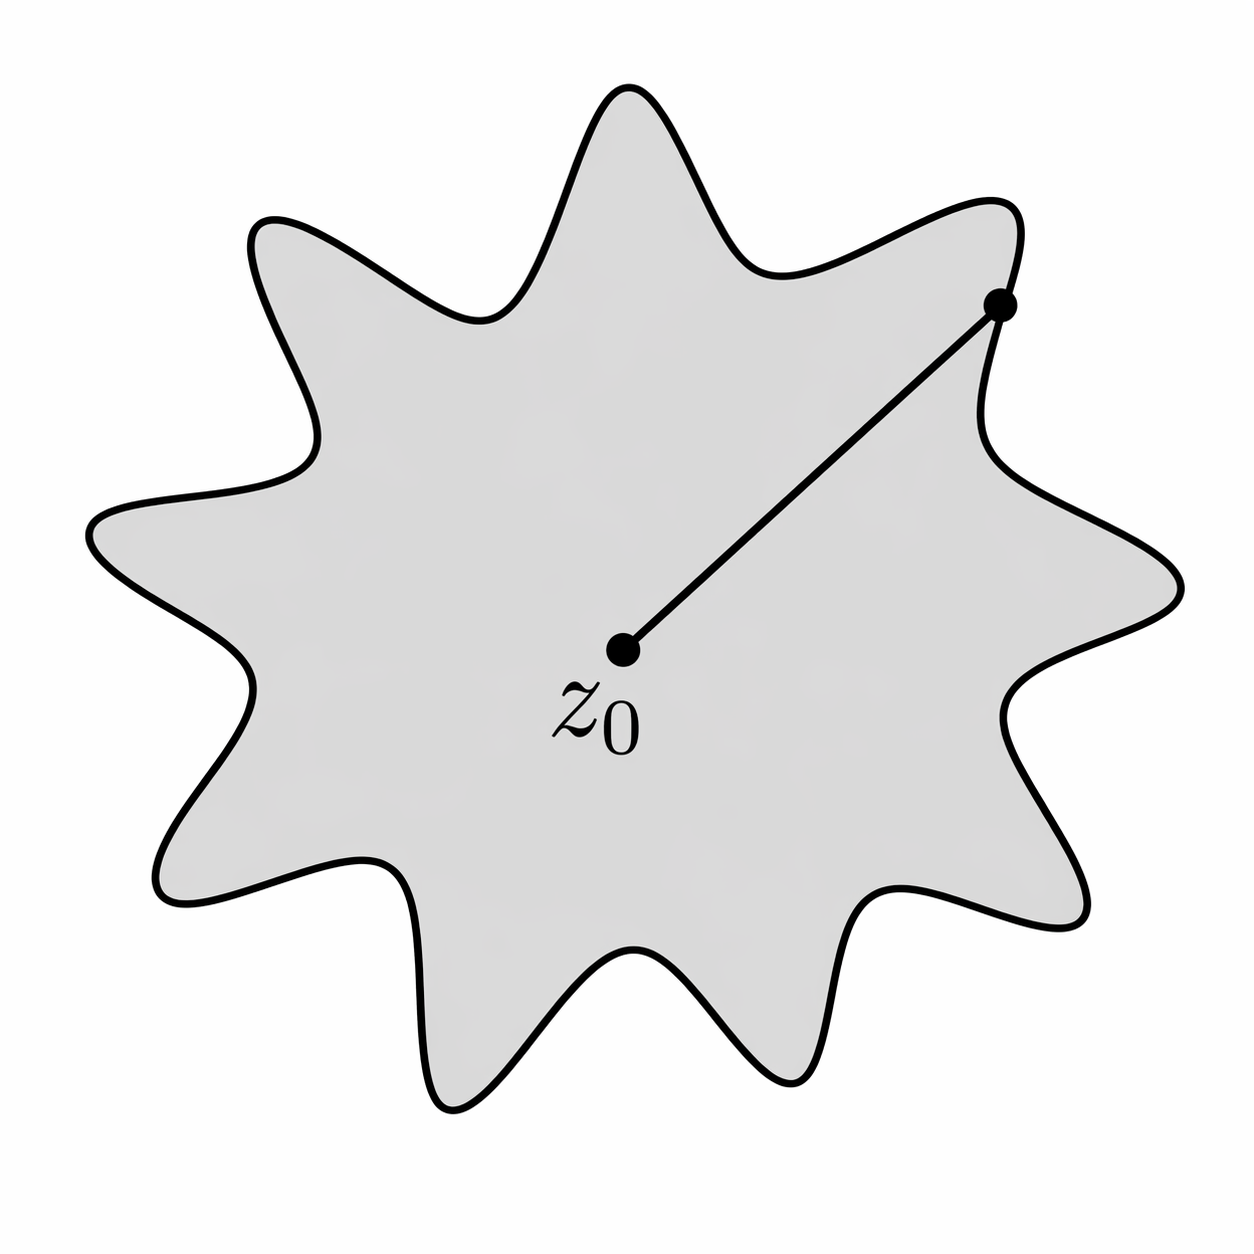
\includegraphics[width=\linewidth]{pictures/Estrellat.png}
        \caption{Conjunt Estrel·lat}
        \label{fig:estrellat}
    \end{subfigure}

    \caption{Exemples dels conjunts definits.}
    \label{fig:comparacion}
\end{figure}

\subsection{Teoremes de punt fix}

En aquesta secció recordem alguns teoremes importants relacionats amb els punts fixos,
així com les nocions bàsiques d'espai mètric, espai normat i espai de Banach que seran
necessàries per a enunciar-los. Per a una exposició general d'aquests conceptes en el
marc de l'anàlisi funcional, es pot consultar \cite{wojtaszczyk}.

\begin{definicio}
    Siga $X$ un conjunt no buit. Una \textbf{distància} en $X$ és una aplicació
\[
d:X\times X\longrightarrow [0,+\infty)
\]
que compleix per a tot $x,y,z\in X$ les propietats següents:
\begin{enumerate}
    \item $d(x,y)=0$ si, i només si, $x=y$,
    \item $d(x,y)=d(y,x)$,
    \item $d(x,z)\leq d(x,y)+d(y,z)$.
\end{enumerate}
El parell $(X,d)$ s'anomena \textbf{espai mètric}.
\label{dist}
\end{definicio}

\begin{definicio}
Siga $X$ un espai vectorial sobre el cos $\mathbb{K}$, on
$\mathbb{K}=\mathbb{R}$ o $\mathbb{K}=\mathbb{C}$. Una \textbf{norma}
en $X$ és una aplicació
\[
\|\cdot\|:X\longrightarrow [0,+\infty)
\]
que satisfà les propietats següents per a tot $x,y\in X$ i per a tot $\lambda\in\mathbb{K}$:
\begin{enumerate}
    \item $\|x\|\geq 0$ i $\|x\|=0$ si, i només si, $x=0$;
    \item $\|\lambda x\|=|\lambda|\,\|x\|$;
    \item $\|x+y\|\leq \|x\|+\|y\|$.
\end{enumerate}
El parell $(X,|\cdot\|)$ s'anomena \textbf{espai normat}.

A més, la norma indueix de manera natural una distància en $X$, definida per
\[
    d(x,y)=\|x-y\|, \qquad x,y\in X.
\]
Així, tot espai normat és també un espai mètric.
\end{definicio}

\begin{definicio}
Siga $(X,d)$ un espai mètric. Una successió $(x_n)_{n\in\mathbb{N}}$ de punts
de $X$ s'anomena \textbf{successió de Cauchy} si, per a tot $\varepsilon>0$,
existeix $n_0\in\mathbb{N}$ tal que, si $m,n\geq n_0$, aleshores
\[
d(x_n,x_m)<\varepsilon.
\]
Un espai mètric $(X,d)$ s'anomena \textbf{complet} si tota successió de Cauchy
en $X$ convergeix a un punt de $X$.
\end{definicio}

\begin{definicio}
    Un \textbf{espai de Banach} és un espai normat $(X,\|\cdot\|)$ que és complet respecte de la distància induïda per la norma. 
\end{definicio}

\begin{definicio}
Siga $(X,d)$ un espai mètric. Una aplicació $f:X\to X$ s'anomena
\textbf{contractiva} si existeix una constant $\lambda\in[0,1)$ tal que
\[
d(f(x),f(y))\leq \lambda d(x,y),
\]
per a tots $x,y\in X$.
\end{definicio}

\begin{definicio}
Siga $f:X\to X$ una aplicació. Un punt $x\in X$ s'anomena \textbf{punt fix}
de $f$ si
\[
f(x)=x.
\]
\end{definicio}

\begin{teorema}[del punt fix de Banach]
    Siga $(X,d)$ un espai mètric complet i siga $f: X \to X$ una aplicació contractiva en $X$. Aleshores existeix un únic punt fix de $f$. 
    
    Podem trobar aquest teorema en \cite[Cap.5, Secció 5.1]{kreyszig}
    \label{banach}
\end{teorema}

\begin{teorema}[del punt fix de Brouwer]

    Siga $f:K\to K$ una funció contínua, on $K$ és un subconjunt no buit, compacte i convex de $\mathbb{K}^n$, sent $\mathbb{K}=\mathbb{R}$ o $\mathbb{K}=\mathbb{C}$, dotat amb la distància euclidiana. Aleshores $f$ té almenys un punt fix.
    
    Una prova d'aquest teorema se pot trobar en \cite[pp. 38-40]{hurewicz} 
    \label{brouwer}
\end{teorema}

\begin{teorema}[del punt fix de Schauder]
    Siga $X$ un espai de Banach, siga $K\subset X$ no buit i convex, i siga $K_0\subset K$ compacte. Si tenim una funció contínua $f:K\to K_0$, aleshores existeix un punt $x_0\in K_0$ tal que $f(x_0)=x_0$.

    Aquest teorema el podem trobar a \cite[pàg. 21]{pata}
    \label{schauder}
    
\end{teorema}


\end{adjustwidth}